\documentclass[full.tex]{subfiles}


% change this line
\graphicspath{ {assets/note7/} }


\providecommand{\notenum}{7}


\begin{document}
    \thispagestyle{firstpage}
    \vspace*{2\baselineskip}
    \section*{Ethereum and Smart Contracts: Enabling a Decentralized Future}
    
    In this note, we will go in depth into what Ethereum is, some technical details on its architecture, how the network and blockchain works, and how the EVM executes Ethereum smart contacts. We will then explore some use cases for Ethereum and see how the technology applies in the real world.
    
    Looking at articles on Ethereum as well as Ethereum's own website landing page, we often come across a plethora of ``buzzwords'' primarily used in publicity campaigns. Decentralized apps, smart contracts, DAOs, Bitcoin 2.0, etc. are all confusing buzzwords used to hype up Ethereum. Our first task will be to demystify Ethereum and to analyze how it works at a high level. Then we will move on to discuss some of the various applications that have been built on Ethereum, and how the emergence of decentralized apps on Ethereum are shaking up markets everywhere.
        
    
    \textit{Note: Unless otherwise specified, use of the word ``blockchain'' or ``network'' refers to the Ethereum blockchain or the Ethereum network.}
    
    \section*{What is Ethereum?}
    
    Looking at it from a very high level, \textbf{Ethereum} is a \textit{decentralized} platform designed to run smart contracts. Ethereum is decentralized in the same way Bitcoin is decentralized: there is no single point of control or failure, and the network is essentially censorship resistant since the resources required to do so would be immense. Additionally, Ethereum is an \textbf{account-based blockchain}, which differs from Bitcoin's UTXO model. It is also useful to think of Ethereum as a \textbf{distributed state machine} in which blocks of transactions are equivalent to state transition functions, which contain information on how to transition between blocks/states.
    
    Ethereum has a native asset called \textbf{ether}, which represents the basis of value in the Ethereum ecosystem. It is used to align the incentives of the various different types of nodes in the system: miners, full nodes, etc. Miners are rewarded in Ether for helping to secure the system once they find the proof-of-work and propagate the first valid block. 
    
    \section*{Ethereum vs. Bitcoin}
    
    Since we already know quite a lot about how Bitcoin works from previous notes, it is useful to draw comparisons between Bitcoin and Ethereum. Ethereum markets itself primarily as a smart contract platform. It is complex and feature-rich (we'll discuss this in later sections) and most importantly, features a Turing complete scripting language. Bitcoin on the other hand is a decentralized asset system primarily used to trade value between users, It is simple and robust. This extends even to its underlying scripting language (Script, or often times just the Bitcoin Scripting Language), which is simple and stack-based, and not at all Turing complete. Why having a Turing complete scripting language is important is because it allows Ethereum developers to define arbitrary computations and programs, all which run on the blockchain. What is important to note is that both Bitcoin and Ethereum have both decentralized assets and scripting languages. They are just designed differently to serve differnt use cases.
    
    The existence of ether is not actually a primary goal of Ethereum. It is used to align incentive within the network. From a game theroretical standpoint, it is important for users to have more incentive to act honestly than to cheat the system. In this way, because the ceators of Ethereum wanted miners to help secure the network via a Proof-of-Work consensus algorithm, they needed to incentivize miners with a block reward of ether. Ether is primarily traded between smart contracts. Another distinguishing factor between Ethereum and Bitcoin is that Ethereum plans to swap out its Proof-of-Work model for an alternative consensus algorithm called Proof-of-Stake, which rewards users for owning a particular percentage/stake of the entire network's capital. We'll go over alternative consensus protocols in a later note.
    
    In terms of implementation details, Ethereum has a target block creation time of about 12 seconds, compared with Bitcoin's 10 minute block creation time. For its version of the Proof-of-Work protocol, it uses Ethash over SHA-256 for its primary cryptographic hash function. Ethash is currently ASIC resistant, but whether or not it stays so in the future is up to debbate. At the time of writing (July 31, 2017), 1 ETH $\rightarrow$ 200 USD, while 1 BTC $\rightarrow$ 2847 USD.
    
    \section*{Accounts vs. UTXOs}
    
    Recall that a Bitcoin user's available balance is the sum of the unspent transaction outputs (UTXOs) for which they own the private keys to the output addresses. Instead of following Bitcoin's UTXO model, Ethereum keeps track of users' available balances by using \textbf{accounts}, each of which consist of an address, a balance, and some optional code. A user's available balance in Ethereum is simply the balance of all the accounts the user has private keys to. 
    
    \begin{center}
    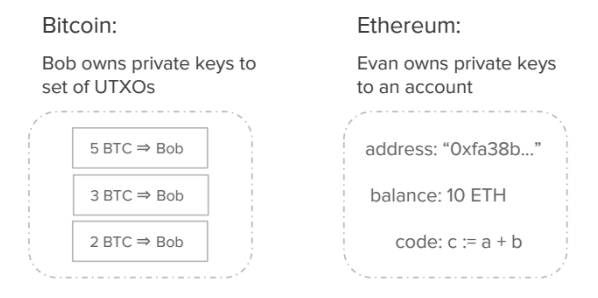
\includegraphics[scale=0.5]{utxo_account}
    \end{center}
    
    The distinction between UTXO and account based models might be subtle for the common user, but it significantly affects the way developers write smart contracts. 
    
    \section*{Ethereum Account Types}
    
    There are two types of accounts in Ethereum. Both are fundamentally similar, except one contains code while the other generally does not. \textbf{Externally owned accounts (EOAs)} are usually owned by some external entity, for example a person or corporation. As do all accounts, they have an address and an ether balance. They can also send transactions to other accounts, whether they be other externally owned accounts or contract accounts.
    
    \textbf{Contract Accounts (Contracts)} on the other hand not only have addresses and ether balances, but also have associated contract code. Code execution for contract code is triggered by transactions or messages (which work as function calls) received from other contracts or externally owned accounts. Contracts have persistent storage for their contract code, as their code, referred to as smart contracts, live and execute distributedly on the blockchain.
    
    \section*{All Accounts == Network State}
    
    In Bitcoin, the state of the network at any point in time is defined by the entire set of UTXOs. In contrast, the state of the entire Ethereum network is defined by the state of all accounts. The entire Ethereum network agrees on the current balance, storage state, and contract code of every single account, and this is the network state that changes for every block in the Ethereum blockchain. It is useful to think of blocks as a state transition function. A block takes the previous network state and produces a new state based on the changes and transactions that have taken pace since the previous block. Every node processes blocks and then agrees upon a new network state based on the changes posed by the blocks. Accounts interact with the network, other accounts, other contracts, and contract state through the transactions that are contained within each block.
    
    \section*{Accounts Rationale}
    
    One of the reasons Ethereum chose to use the account model rather than Bitcoin's UTXO model is that they wanted to save space. Instead of having to save every UTXO to determine one's balance, Ethereum just has to update each account's balance after every transaction. The account model is also more intuitive when writing a smart contract. It's much easier to make a program that transfers value between accounts with a balance, rather than having to constantly update a UTXO set to compute a user's available balance. 
    
    \section*{Smart Contracts}
    
    Ethereum is smart contract platform, but what exactly is a smart contract? Google says that a contract is ``a written or spoken agreement...that is intended to be enforceable by law.'' For example, a futures contract is an agreement to sell a particular asset at a predetermined price at a specified time in the future. If a contract goes well, assets exchange hands as specified, and all goes well. If not, parties associated with the contract could potentially sue and go to court, which would decide the lawful outcome of the situation. Similarly then, we can define smart contracts as ``code that facilitates, verifies, or enforces the negotiation or execution of a digital contract.'' In order for smart contracts to function properly, they must be executed by a trusted entity. Instead of a trusted third party, trust can be reached by using a distributed and decentralized network. Previously we mentioned that the blockchain is a structure that establishes trust, so the logical conclusion is to take smart contracts and encode them onto the blockchain -- and that's exactly what Ethereum does. Smart contracts on Ethereum run in the context of the global state of the network, established by blocks, and everyone on the Ethereum network agrees on what these smart contracts do.
    
    \section*{What is a Smart Contract?}
    
    In Ethereum, smart contracts are executed by the network itself. Every single node in the network (full nodes, miners, etc.) execute the code in each contract when a function is run. This happens in lockstep across all nodes at the same time, meaning that every node is executing the same step at the same time, maintaining a parallel redundancy. This ensures that no one can violate the contract, because everyone in the network agrees on what the contract should do. Network consensus removes the need for a trusted third party, and this removes any worries about maliciously altered contract execution. Like in the case of Bitcoin, we can assume that Proof-of-Work solves all these problems, and for someone to successfully violate a contract, they must first subvert the entire network.
    
    One way to think of smart contracts is to imagine them as autonomous agents that live inside of the Ethereum network. The way we trigger them and to have them react to the external world is to ``poke'' them with transactions, which call certain functions defined in their smart contract code. Smart contracts have direct control over their own internal ether balance, internal contract state, and also permanent storage, so these could be potentially changed based on how a smart contract is designed to react to transactions.
    
    Ethereum smart contracts generally serve four purposes. Firstly, contracts can be used to \textit{store and maintain data}. This could be useful in representing something useful to users or other contracts, and could for example be used to build another token currency within Ethereum, keep track of an organization's membership, or maintain a domain name registrar. Other contracts \textit{manage contract or relationship between untrusting users}, and these are commonly used when parties do not necessarily trust each other, but want the same code to be executed by all parties. Such contracts find use in financial contracts, escrow, and insurance, where it is easy for a party to attempt to cheat. In which case, a single, common source of truth -- the Ethereum network -- executes the code and helps maintain integrity. Some contracts exist to \textit{provide functions to other contracts}, and do not talk directly with normal users. Examples of such contracts are those that serve as software libraries. Lastly, some contracts offer \textit{complex authentication} functionality. Contracts could implement M-of-N multisignature access, where $M$ number of nodes of a set of $N$ are needed to make decisions -- think multisig wallets and board members coming to consensus. While we identified only four general purposes, there are many contracts in the Ethereum network that are a combination of the four classes mentioned.
    
    \section*{Minimum Viable Token}
    
    Next, let's look at a basic sketch of a smart contract that defines the functionality of a new token currency, called PhilipToken. As with most other smart contracts, PhilipToken is written in an Ethereum specific language called Solidity, and compiles down to EVM (Ethereum Virtual Machine) bytecode.
    
    \begin{center}
        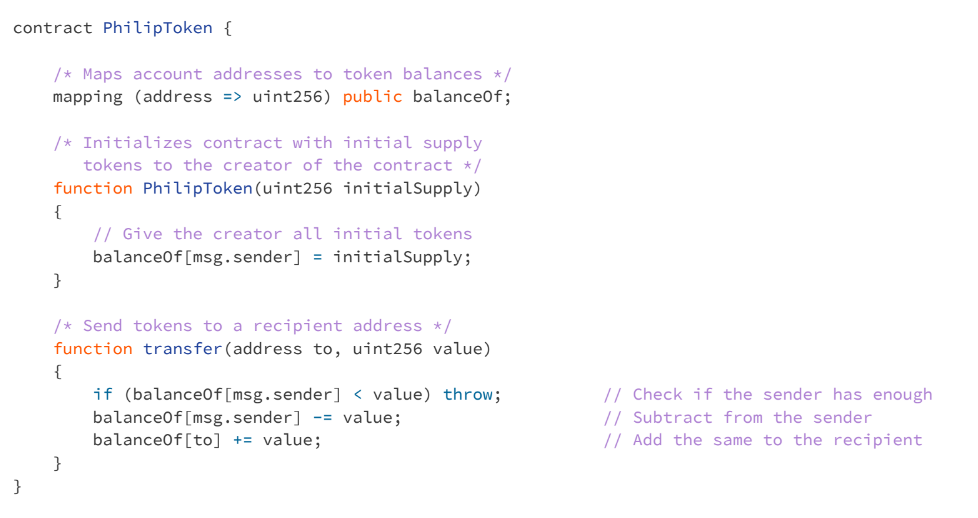
\includegraphics[scale=0.5]{mvt}
    \end{center}
    
    In PhilipToken, we can instantiate the contract in such a way as to give all initial tokens to the creator. This seeds PhilipToken and defines the total amount of PhilipToken that is available. PhilipToken contains a mapping from address to token amount, and this is useful when keeping track of who owns how much token. After initializing a new PhilipToken instance, the creator can then transfer PhilipToken to other addresses. We can see in the bottommost function that if the sender has enough token, the sender's balance decreases by the transfer amount, and the recipient's balance increases by the same number. If the sender does not have sufficient funds, then an error is thrown.
    
    While this example is very basic, it outlines the potential of Ethereum as a platform. With a few lines of code, we have defined a new token currency that can be traded between any Ethereum users. Because the network is decentralized and distributed, the currency is secure, and thus immune to censorship or other attacks by governments.
    
    \section*{Ethereum Virtual Machine}
    
    Contract code on Ethereum is run on the \textbf{EVM (Ethereum Virtual Machine)}. The contract code we saw in the previous section was written in a language called Solidity, one of many languages developers can choose to write Ethereum smart contracts in (other languages are Serpent, LLL, Viper, etc). Contract code written in these higher level programming languages compiles down to EVM bytecode that is executed on every node. EVM bytecode is a low-level, stack-based bytecode language similar to that of the JVM (Java Virtual Machine.) Every Ethereum node runs the EVM on all of the transactions in a block as part of its verification procedure, to update their internal state to match the new network state. The diagram below illustrates how contract code compiles down to EVM bytecode that is executed on all nodes in the network.
    
    \begin{center}
        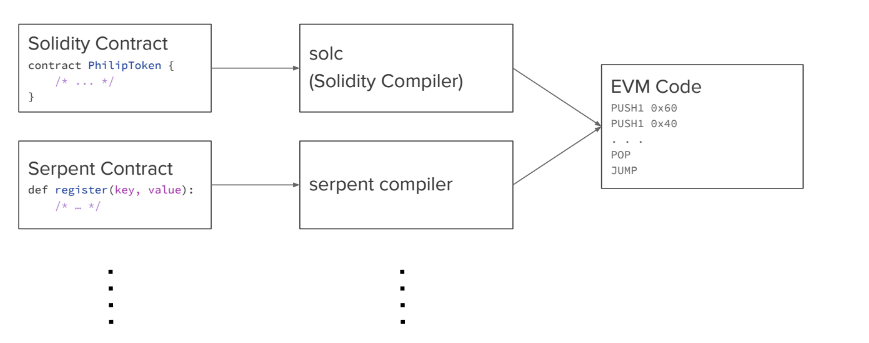
\includegraphics[scale=0.5]{evm_pipeline}
    \end{center}
    
    The EVM is essentially the underlying state transition mechanism for each of the nodes in the Ethereum network. We start off with the current block state, the gas required for code execution, the memory of the contract, the transaction that's calling the contract, message metadata, the code of the contract, stack of the contract, and the program counter. All this data is fed to the EVM, which calculates a new block state with all the updated account info on balances and long-term storage, and however much gas remains from the execution. 
    
    \begin{center}
        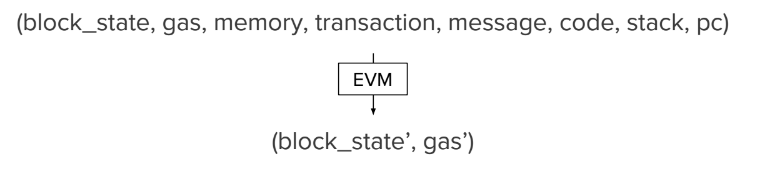
\includegraphics[scale=0.5]{evm_transition}
    \end{center}
    
    \section*{EVM Design Goals}
    
    Some of the funamental design goals of the EVM are simplicity, space efficiency, determinism, specialization, and security. The EVM code was designed to be as simple as possible, to minimize the number of op-codes available by making them as low-level as possible. By making the set of op-codes smaller, we can minimize the amount of space required to represent the op-codes in bytecode, so that gives us a bonus in space efficiency. Determinism ensures that every node executes EVM code in the same exact way, regardless of the underlying architecture of the node. The same input state should always yield the same output state. The EVM should also be specialized, meaning that it should be ale to easily handle common operations such as those used in the underlying cryptography of Ethereum. The EVM must handle 20-byte addresses and custom cryptography with 32-byte values, modular arithmetic, and block and transaction reading with speed and accuracy. Security ensures that there is no way to overflow the EVM and take over a node, for example. Gas cost makes the EVM realistically non-exploitable. We'll talk about how this happens in the next section.
    
    \section*{EVM Gas and Fees}
    
    One immediate concern with the design of Ethereum smart contracts is that if they are executed on all nodes, what if someone writes a contract that executes an infinite loop? Assuming someone writes a transaction to this contract, all nodes would essentially be stuck executing the same loop forever, halting the network. This would essentially be a denial of service attack, and would immediately cripple the network. By the \textit{halting problem} of compatibility theory, it is impossible to determine ahead of time whether a written contract will ever terminate. How do we solve this network-breaking problem?
    
    Ethereum's solution is to implement the concept of \textbf{gas}, which every contract requires in order to ``fuel'' contract execution. Every EVM op-code requires some gas in order to execute. In building a new transaction to a contract, one must specify in the transaction the \textit{startgas}, or the maximum quantity of gas they are willing to consume in the transaction. \textit{Gas price} specifies the fee in ether the transaction is willing to pay per unit gas -- in other words, the gas to ether exchange rate. 
    
    At the start of a new transaction, the user calculates $startgas * gasprice$, and this amount in ether is subtracted from the user's account balance. If the contract successfully executes, any remaining gas is refunded to the user's balance. If the contract execution runs out of gas before it finishes, then the execution reverts. Also, the initial amount of ether the user put in, $startgas * gasprice$, is not refunded. Therefore, it is important to always overestimate the amount of gas required to execute a contract. 
    
    Looking back at the infinite loop problem, we can see that it is technically possible to write an infinite loop and launch a denial of service attack. The attacker would just have to pay enough ether to fund the attack, and this amount is so large that it realistically is not a threat to the Ethereum network. You can think of purchasing gas as purchasing distriuted, trustless computational power. Like how attackers in Bitcoin would have to use a lot of capital to get enough hardware to subvert the network, attackers in Ethereum must obtain enough Ether to use as gas to fuel their infinite loop denial of service attack. 
    
    \section*{Ethereum Conclusions}
    
    One important idea to grasp about Ethereum is that it is not designed to prioritize efficiency of computation. In fact, when compared with the average computer, the Ethereum virtual machine is terribly slow. Ethereum is optimized for distributed and trustless execution. All transactions are run across all nodes in the network, making Ethereum redundantly parallel. This in turn is an efficient way to reach consensus on the system state without needing to trust a third party. Furthermore, because contract executions are redundantly replicated across nodes, computation is expensive. The cost associated with executing a contract creates an incentive not to use the Ethereum blockchain for computation that can be done off chain. 
    
    \section*{Smart Assets}
    
    Now we'll dive into some of the use cases of smart contracts in Ethereum. With our PhilipToken, we have seen how easy it is to implement a new token system in Ethereum. It is essentially modeled after a database with a single operation: to ensure that Alice has enough money to pay Bob. If so, subtract that amount of token from Alice and give it to Bob. All this can be done in a few lines of code, as can be seen in PhilipToken, and also in the Ethereum whitepaper:
    
    \begin{center}
        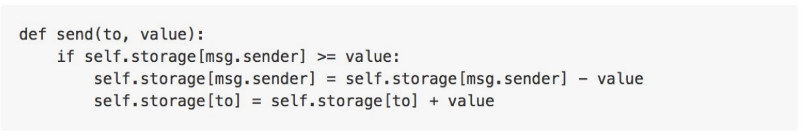
\includegraphics[scale=0.5]{smart_assets}
    \end{center}
    
    \section*{Public Registry/Pubic Database}
    
    Smart assets contain a database to keep track of how much token each address has. We can use the same idea to build a public database that can be used as a domain name registry for example. We start to build this DNS system by mapping domain names to their corresponding IP addresses, through which they are hosted. Having this database on the Ethereum blockchain makes the data stored in it immutable, since everyone has to come to consensus about it, and could easy cross check the mappings. Such a system would be easy to implement on Ethereum too, as shown in the Ethereum whitepaper:
    
    \begin{center}
        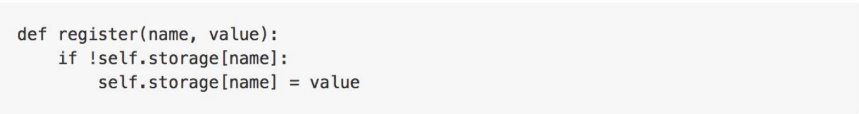
\includegraphics[scale=0.5]{public_registry}
    \end{center}
    
    \section*{Crowdfunding and Incentivization}
    
    Another use case for Ethereum is for crowdfunding. ``Ether-on-a-stick'' is a smart contract that allows Ethereum users to put a bounty on the completion of arbitrary tasks. Contributors pool money into a smart contract that pays out to a specified recipient if and only if contributors vote that the task was indeed complete. An example use case could be if a company is polluting a local river, and nearby residents are bearing a negative externality. If the local government is slow and unresponsive, and the residents are willing to pay, the residents could pool money together to incentivize the company to clean up the river. If the company cleans up the river, the contributors could come to consensus over whether the river was cleaned up, and the smart contract would then pay out to the company. ``Ether-on-a-Stick'' implements a dominant assurant contract and solves the free rider problem.
    
    \textit{(Note: ``Ether-on-a-Stick'' was a hackathon project of Blockchain at Berkeley members Max and Philip)}
    
    \section*{Smart Energy Grids}
    
    Imagine that a neighborhood has a smart energy grid. There might be some imbalances in energy (heat, electricity, etc.) across the community. House A might have excess heat, while House C may be too cold. House A could sell its excess energy to House C, cancelling out the energy difference. In other words, there would have to be an energy market. The energy market would save both parties, House A and House C in this case, money, and would make the entire community as a whole more power efficient. 
    
    The problem with such a system is that there is no existing infrastructure that supports the direction of electricity sales. Energy infrastructure currently flows unidirectionally, from the utility companies to individual houses. Utility companies generally do not want to build smart grid infrastructures since this would entail less revenue for them, since energy sales between households would cut into their profits. The government also has little to no incentive to help build these smart grids. Only the household peers would benefit from the smart grid infrastructure. 
    
    The solution would be to set up an Ethereum smart contract for financial commitments. The smart contract could help coordinate the development of the smart grid in a neighborhood without individual houses having to trust one another. A contract would read something like this: ``I, House A, commit \$10,000 to building this infrastructure. If House B and House C also commit the same amount, the total amount will go to this contractor to begin construction on our smart grid, and the total amount can only go to this specific contractor.'' The Ethereum blockchain thus serves as a coordination layer for the community's decision. Households fall back onto the blockchain when coordination cannot be found via a central entity or government. What was originally a social problem can now be solved technologically with the Ethereum blockchain. 
    
    \section*{Decentralized Prediction Markets}
    
    The idea of decentralized prediction markets draws on the wisdom of crowd-sourced knowledge in an attempt to predict or forecast the future. Essentially, these would work by first allowing market makers to create an event. For example, they could make one for ``Who will win the 2020 US Presidential election?'' Events for decentralized prediction markets must be public and easily verifiable, with a set due date. This is because anyone must be able to verify the result, and also we need to know when to stop taking predictions. Participants in the decentralized prediction market would then buy shares of Trump or Zuckerberg, and pay a small fee. On election day, random oracles on the network would vote on who won, essentially bringing in external data from the real world into the blockchain. Oracles who voted with the majority collect the fee that was paid by the participants. Otherwise, the oracles are penalized, and could potentially lose their status as an oracle. Shareholders who voted correctly would be able to cash out on their bet after election day.
    
    The share price for each market accurately represents the best predicted probability of an event occurring. Say that the shares for Trump and Zuckerberg are currently trading at 0.50 USD. This roughly equates to Trump and Zuckerberg having an equal probability of winning the 2020 election. However, if you know somehow through secret insider information that Zuckerberg's chance of winning is actually 70\%, you could buy Zuckerberg shares until the share price goes up to 0.70 USD. Therefore, you have acquired shares that were worth 0.70 USD at the price of 0.50 USD. Based on the expected profit then, you have made money.
    
    The powerful potential behind decentralized prediction markets is that it allows people to bet on not only political events, but practically anything else as well. It's a cost efficient way to buy information on a future event. Instead of hiring pundits and experts, you could create a market for your event and let the wisdom of the crowd generate a prediction for you. For example, you could set up a decentralized prediction market for determining if a new movie will flop or not. Users betting for and against this event create liquidity for that particular prediction. Hollywood insiders who know whether the movie will flop or not would then be incentivized to vote on whichever side of the prediction is beneficial to them. Then, you have essentially bought this insider information from them.
    
    Decentralized prediction markets also find use cases in hedging and insurance. For example, whenever you buy fire insurance, you are betting that your house will burn down, otherwise you lose the funds you invested into the fire insurance. You could create a market asking the network to predict whether your house will burn down, and vote yes, because you're betting that your house will burn down. Insurance companies could then take sides on this prediction, depending on their expert analysis and judgment. If they predict that your house will not burn down, and it does, then you receive all the money that was pooled in. Of course there would be moral concerns with such a prediction market, but as an example, this shows the power of decentralized prediction markets. Taking the example a step further, it is even possible to implement an entire insurance liquidity pool onto a smart contract, avoiding the costs of offices, employees, etc.
    
    Augur is one of the biggest decentralized prediction markets currently in operation. The way they secure their codebase uniquely leverages their product to detect bugs. First, they set up a security bug bounty on their decentralized prediction market. ``Will someone be able to steal the money in this prediction market?'' Augur then bets heavily against this prediction to create a financial incentive for someone to find a vulnerability. If someone successfully finds a vulnerability, they would buy affirmative shares to reflect their belief, and then perform their hack. Once the hack is detected, the individual would profit.
    
    Another way to use a decentralized prediction market is to signal -- essentially the economic term for ``put your money where your mouth is.'' You can demonstrate your commitment to something by showing you will take a large financial loss if you miss your commitment. For example, say you are the leader of a huge Kickstarter campaign, and investors are worried that you will delay the launch date. You could then create a vote for ``Will my Kickstarter campaign launch on time?'' and bet heavily that you will in fact launch your product on time. If you lose, then you take a huge financial loss. However, this shows that you are confident that you will carry through with your commitment, since you are betting so much money and willingly exposing yourself to so much financial risk. 
    
    There are many benefits of creating decentralized prediction markets -- the first being that there are no restrictions on market creation. We previously mentioned that prediction markets could be created for not only politics, but for a variety of other subjects as well, opening the possibility of hosting such functionality as the advanced examples we discussed. Arbitrary markets allow for much wider range of applicability. The caveat however is that we need a defense mechanism against unethical or illegal markets. Augur solves this problem by having oracles vote on whether prediction markets are unethical or undecidable. This prevents assassination markets or other markets with moral danger from popping up. Another benefit of decentralized prediction markets is that they create a shared liquidity pool. There's no reason why the same market should exit in multiple countries. Decentralized prediction markets could be used as a back-end service to take votes for variety of different applications. Other benefits are that decentralized prediction markets are censorship-resistant, because of properties of the Ethereum's distributed network, and also allow for automatic, trustless payments through the smart contract code.
    
    \section*{Decentralized IOT}
    
    Ethereum's support for general smart contracts lends itself nicely to IoT (Internet of Things) because now we can automate the communication of various IoT devices on a distributed network. Filament is a company at the forefront of designing the ``Blockchain-based decentralized Internet of Things.'' They build IoT sensors intended for industrial applications that are connected to one another via an ``ad hoc mesh network.'' Sensor units with a 10 mile range, and include a battery that lasts for years. No internet connection is required, as sensors are connected using a mesh network. One of the use cases of Filament's solution is for the agriculture industry. Units could be deployed across vast farmlands and could be used to transfer important information in a secure way.
    
    An interesting note is that blockchain is only one aspect in Filament's entire technologica stack. Blockchain is only used to keep track of name-address bindings for each individual sensor. This is then used to discover new devices on the network and to verify the authenticity of certain bindings. The name-address bindings are incorruptible because of the blockchain's property of immutability. Contrast this with a central database that could be maliciously altered with a single point of failure. Thus, Filament is a great application of decentralized tech especially because of its emphasis on resilience and dependability. Data for the bindings is duplicated across on all connected sensor units, increasing data redundancy, which entails increased durability.
    
    \section*{After Hours Trading}

    24 hour stock trading would be convenient, and given that our world is highly digitized, why does it not exist? After hours trading has not taken off because it faces a problem in liquidity. There is not enough liquidity, so prices are more volatile and destabilizing. The government sees this as dangerous, and passes regulation that restricts trading to only using limit order. This is only sustainable at larger brokerages where there is enough stock to sustain any kind of market. It's nice to have convenience, but it's more important to have a better price discovery in the market. 
    
    A solution to enable after hours trading might be to create a blockchain-based asset exchange with legal bindings. Brokerages can let users ``withdraw'' their stock into stock tokens on a blockchain. The stock is then subtracted from the user's account, and the brokerage holds it in the meantime. The brokerage then writes a legal contract saying that: ``Anyone who proves that they own a stock token is eligible to redeem it for a stock I am currently holding.'' These legal contracts make it such that tokens on the blockchain are backed by real stocks. Now you can create a trustless blockchain-based stock exchange that allows users to trade stock tokens, which can be redeemed for actual stock via the legal contracts written by the brokerages.
    
    The result is that after hourus trading is enabled with very little cost. Anyone on the Ethereum network can now use their ether to buy stock tokens and trade after hours: 24/7/365. Multiple brokerages can participate and create a shared liquidity pool. In addition, these brokerages don't need to trust each other, as the blockchain ensures that all the rules of asset management, deduplication, and stock trading in general been encoded in a smart contract, are being carefully followed. Anti money laundering is enforced when traders redeem their tokens. All trading history is transparently logged on the blockchain, so malicious traders can be caught with evidence.
    
    \section*{Decentralized Autonomous Organizations}
    
    The last Ethereum use-case we are going to cover is something called a \textbf{decentralized autonomous organization (DAO)}, which is an organization governed entirely by the code within smart contracts. DAOs create and vote on proposals based on their design, and could even theoretically replicate entire businesses on the blockchain. After all, functionality such as decision making and making payments is easy to create on Ethereum. Such businesses would have uncertain legal status however. The general idea of DAOs can be summarized by the phrase ``code is law'' -- that is, trust in math and code rather than in governments and institutions.
    
    Some issues with DAOs are that they are hard to edit once they are deployed. Smart contracts are immutable after all. A possible solution would be to implement a Child DAO, but historically this has not been secure, especially when considering this was the cause of the crash of TheDAO. TheDAO was the largest crowdfunded project in history, which at the time raised more than \$150 million in Ether. It was hacked in June 2016, when more than \$60 million worth of Ether was stolen (10\% of the Ethereum market cap.) 
    
    The use of a DAO can be seen in Dash, a privacy-centric cryptocurrency, where a certain percentage of the mining reward goes to a set of ``master nodes'' which decide on changes to be made. Dash thus creates a self-sustaining, decentralized ecosystem. Some other cryptocurrencies have something called a ``founder's reward'' which allocates some award to a specific group of people, presumably the founders and creators of the currency, making the entire system centralized. Dash refuses this temptation in an attempt to make a more pure decentralized, privacy-centric cryptocurrency solution.
    
    \section*{Limitations on Blockchain Tech}
    
    One of the main limitations of blockchain technology is that there is \textit{no trustless way to access outside data}, creating the effect of blockchains existing within silos, or having to take the risk of trusting others. Blockchains often times must rely on \textbf{oracles} to provide information from outside the blockchain. We saw an example of this in the decentralized prediction markets section. The problem is that we must find a way to trust these oracles. A potential solution is \textbf{proven execution}, which involves an oracle proving that an HTTP request for useful data existed at a certain period of time, and that they did not manipulate it before sharing it with the blockchain. Tools like Oraclize offer proven execution implementations for communication between Ethereum smart contracts and a variety of Web APIs. Oraclize uses TLSnotary, which is a modification of the TLS (transport layer security) protocol to provide cryptographic proof of receiving an HTTPS page. Another potential solution to the problem of getting data off-chain onto the blockchain could be to create an \textbf{oracle network}, which is what Augur does in its decentralized prediction markets. A drawback however is that you would have to build a consensus protocol into the oracle network in order to ensure security, and this would essentially mean you would have a consensus protocol (for the oracle network) built on top of another consensus protocol (that of Ethereum). There are a number of edge cases that arise from consensus protocol layering that are difficult to test. 
    
    Another limitation of blockchain technology is that there is \textit{no way to enforce on-chain payments}. It's difficult to impllement financial products such as loans and bonds because they would require money be held on the blockchain to ensure payment. For example, you cannot issue loans via contract and trustlessly have the sum returned to you, since trust is fundamental to borrowing money. Intuitively, with loans, we usually pay an interest because there default risk, or a risk that someone will not be able to pay back their loans. A compromise involving the blockchain that we can implement is a decentralized reputation system, or a credit rating system. This would give some level of trust to the nodes with higher reputation/credit.
    
    The final limitation of blockchain technology we will mention is that \textit{contracts cannot manipulate confidential data}. If you create a smart contract to handle confidential data, having it on the blockchain means that everyone else on the network potentially has access to your data. You could encrypt the data before putting it onto the blockchain, but you would have to decrypt the data locally. Manipulating data directly on the blockchain after encryption would be incredibly difficult, as the only solution as of now would be to use \textbf{homomorphic encryption}, but such technology is still being designed.
    
    \section*{Essential Properties of Killer Blockchain Apps}
    
    With so many use cases of Ethereum and blockchain technology, it is often difficult to identify well deigned applications from ones that are not, especially with all the hype going around. For every application, it is helpful to ask yourself: Why is using a blockchain better than using a centralized database? Understanding why blockchain is so good at what it does, and how sticking a blockchain into any ordinary application could make them worse, is a good exercise in identifying killer blockchain applications. The following is a list of some essential features and properties where blockchains excel over the standard centralized database.
    
    Blockchains are really good at creating trustless environments that need consensus or coordination. It's by the design of blockchains and their underlying consensus algorithms that enable them to be decentralized, distributed, and trustless. Think of Ether-on-a-Stick, in which community members can come to consensus over whether a company has cleaned up a nearby polluted river, or smart grids, which have to come to consensus over the state of the current energy market. 
    
    Blockchains also allow for disintermediation and censorship-resistance. Cryptocurrencies allow for truly peer-to-peer payments through the blockchain, that bypass the need for a central authority managing and tracking where all the money flows. Blockchains' property of immutability means that it's costly for anyone to try to rewrite the block history, and this property naturally extends to encompass censorship-resistance, as we saw in the last note in the section on censorship attacks.  
    
    Data collected and managed by people can often be faulty, and it might be that markets can handle data with a higher degree of accuracy. Writing a smart contract with a set of rules on how to handle data means that the data is ``correct by design,'' because the blockchain guarantees that any rules defined by the smart contract will be enforced. Data generated can thus be traceable, and also have a high degree of authenticity because it was agreed upon by the network. The only caveat is that data entering the blockchain must also be correct -- a problem for oracle networks or similar solutions to handle, and not necessarily a shortcoming of the blockchain infrastructure.
    
    The combination of money and code gives rise to the concept of easily programmable money. (How surprising!) Since blockchains are traditionally good at handling cryptocurrencies, and that smart contracts allow us to programatically deal with money, it is easy to see how automated payments could be built. This application of blockchain technology would find use in machine to machine payments on the Internet of Things. IBM ADEPT is a project by IBM and Samsung that attempts to create a blockchain-powered Internet of Things. Programmable money is also particularly useful for micropayments. For example, when the Lightning Network -- or another equally fast extension to the blockchain -- is in place, automated micropayments with tiny transaction fees could be implemented. Currently, micropayments are not realistic because miners prioritize transactions with larger transaction fees.
    
    As we saw with Augur and also Ether-on-a-Stick, blockchains also give us ways of creating incentives. People and organizations are after mainly profit as one of their primary incentive, and blockchains conveniently feature value in the form of cryptocurrencies. Cryptocurrencies could be used to incentivize others to provide information or truth, or to take a particular action. Additionally, smart contracts give us away of creating robust and secure management systems, as we see with a majority of smart contracts that have internal rules and code that the network confirms. This however often breaks down at the interface with the real world, as that is when you have to rely on trust and not the guarantees of the blockchain. Building on smart contract rules and management, blockchains can also create new governance models. Although this is a relatively new field, examples in decentralized autonomous organizations (DAOs) have proven that this is effective, at least on-chain.
    
    
    \section*{Conclusion}
    
    Contrast all the perks of blockchain technology with the perks of having a centralized database and you realize that there are use cases for both of them. It's not realistic to slap a blockchain onto an existing application and instantly have that app upgraded. Centralized databases are still better than blockchains at deep integration and creating a great and cohesive user experience. Facebook owns all of our data, and because they have all this data on their own servers, they can run machine learning tools on our data to tailor what we see on our Facebook news-feeds to what we usually generally interact with. This isn't practical on a blockchain solution because blockchains aren't efficient enough. (In fact, blockchains are probably the world's worst database -- it's only selling point is that it is decentralized and distributed, and allows for this handy thing called consensus without the need for trust.) Centralized control also allows for clearly defined read/write permissions over data. Blockchains being distributed means that everyone has access to all the data. Finally, not everything can be done on a blockchain (yet), and often times problems that were unaccounted for during project design need human level interaction to solve. One of the reasons why we're a long way from a ``decentralized Airbnb'' is that potential disputes between users are hard to predict and write into logic onto smart contracts. Instead, it is more efficient to have actual people manage this unpredictable human level complexity on a case-by-case basis.
    
    The conclusion is that while blockchain technology and distributed tech as a whole is poised to lead to a new world of decentralization, it is important to consider the properties that make distributed solutions so great in the first place. Blockchains are great, but not applicable to everything at their current state. 
    
 
    
    % BEGIN KEY TERMS
    \newpage
    \thispagestyle{firstpage}
    \vspace*{2\baselineskip}
    \section*{Key Terms}
    \noindent A collection of terms mentioned in the note which may or may not have been described. Look to external sources for deeper understanding of any non-crypto/blockchain terms.
    \begin{enumerate}
        % edit within here
        \item \textbf{VOCAB WORD} --- Definition. % format
    \end{enumerate}
    % END KEY TERMS
\end{document}